\chapter[Introdução]{Introdução} \label{cap:introducao}
% \addcontentsline{toc}{chapter}{Introdução}

A democracia digital é resumida por \citeonline{penteadoencontro} como o uso da Internet para consolidação da democracia.
Esse uso tem acarretado em um crescente número de discussões acerca de temas políticos, o que permitiu que interessados na área analisassem 
esse fenômeno e observassem uma polarização das mensagens trocadas nas redes sociais \cite{empurrandojuntos}.

\citeonline{empurrandojuntos} afirmaram que as discussões realizadas, principalmente em redes sociais, 
acabavam refletindo sempre a opinião da maioria e que as pessoas estão sempre presentes em uma bolha de opinião. 
Isto é, os algoritmos dessas plataformas selecionam o conteúdo a ser apresentado de acordo com o comportamento anterior,
no qual foi coletado a opinião deste usuário.
Dessa forma, essa polarização dificulta a explanação das ideias da minoria e restringe a apresentação de novas ideias ou pensamentos diferentes 
para quem usa essas redes sociais. 

Observando esse aspecto, o Instituto Cidade Democrática apresenta a ideia da plataforma ``Empurrando Juntos'' cujo objetivo 
é dar voz para a minoria e tornar as discussões mais efetivas para os seus propósitos \cite{empurrandojuntos}.

A ideia é que um usuário possa criar conversas e participar de conversas criadas por outros usuários. Essa participação 
acontece de duas formas: comentando em uma conversa ou votando em um comentário de outro participante. Entende-se por voto
o ato de concordar com o comentário realizado (uma espécie de \textit{like}) ou discordar do comentário. Além disso, é permitido
que o usuário pule aquele comentário, ou seja, não atribua nenhum tipo de voto \cite{empurrandojuntos}. 

Com os votos realizados, a ideia é agrupar pessoas que responderam de maneira parecida, ou seja, concordaram e
discordaram dos mesmos comentários. Com os grupos formados, é possível ver a convergência e divergência de opiniões, 
prover ao usuário uma visão ampliada das opiniões acerca do assunto e promover a interação entre os usuários com 
pensamentos divergentes.

% 
% Para o ``Empurrando Juntos'' foi prevista uma arquitetura cliente-servidor a fim de possibilitar a criação de aplicações e
% aplicativo. O lado servidor, é composto por dois módulos: o módulo de serviço e o módulo \textit{Math}. 
% 
% Atualmente, na plataforma foi implementado somente o módulo \textit{Math}, responsável por realizar o agrupamento em tempo real, 
% ou seja, conforme as pessoas votam são formados ou modificados os grupos. 
% Isto é, não há estabelecimento prévio dos grupos somente se sabe que os usuários têm dados em comum, que são os votos nas conversas,
% mas , para que os usuários façam parte deles. Essa característica
% determinou a implementação do módulo utilizando a técnica de clusterização.
% 
% Uma \textit{Application Programming Interface} (API), é uma interface que expõe os seus componentes como um serviço, 
% permitindo que outras aplicações interajam com esses componentes \cite{wagh2012comparative, understanding_web}. 
% Essa arquitetura de serviços possibilita o compartilhamento dos dados armazenados com as aplicações que consomem o serviço. 
% 
% O uso de uma API permite a convergência de informações e disseminação da sua proposta por meio de seu uso em diversos tipos de sistema.

% 
% Atualmente, novas plataformas têm surgido com o intuito de melhorar a efetividade das discussões promovidas na Internet. 
% Uma dessas plataformas é o Empurrando Juntos. A ideia é mudar o fluxo de comunicação que tem se formado nas redes socias, 
% a fim de permitir que todos sejam ouvidos e privilegiar aqueles que se encontram na minoria, 
% os quais perdem a visibilidade das suas mensagens \cite{empurrandojuntos}. 
% Em suma, a plataforma "é um aplicativo de conversa na rede com uma interface minimalista de participação que identifica e 
% exibe grupos de opinião e propostas a partir dos dados de participação" \cite{empurrandojuntos}.
% 
% Segundo \citeonline{violence_against_women}, o termo violência contra a mulher trata de
% diversos atos de abuso e violência baseados no gênero, ou seja, dirigidos à mulheres e meninas ao longo da vida.
% De acordo com o estudo da \citeonline{violence_global}, dos diversos tipos de violência existentes, a violência doméstica, ou proveniente do parceiro,
% e a violência sexual, proveniente de um indivíduo diferente do parceiro, são as formas de violência que prevalecem.
% 
% A pesquisa relatada pela \citeonline{violence_global} mostra que 35\% das mulheres no mundo já vivenciaram uma situação
% de violência pelo física e/ou sexual pelo parceiro e violência sexual por outro indivíduo. No mundo, 38\% dos homicídios de mulheres são cometidos 
% pelos parceiros das vítimas.
% 
% No Brasil, de acordo com o Sistema de Informações sobre Mortalidade (SIM), entre 1980 e 2013, 106.093 mulheres foram vítimas de homicídio, representando em 2013 uma taxa de aproximadamente 13 homicídios femininos
% diários \cite{mapa_violencia_2015}. 
% No primeiro semestre de 2016 foram contabilizados 555.634 atendimentos na central de denúncias 
% de violência contra a mulher, de acordo com o levantamento feito pela Secretaria de Políticas para as Mulheres (SPM). 
% Aproximadamente 54\% dos atendimentos foram para prestação de informações. De acordo com \cite{portal_180}, aproximadamente 13\% dos atendimentos, 
% são relatos de violência física (51\%), psicológica (31,1\%), moral (6,51\%), patrimonial (1,93\%), sexual (4,30\%), cárcere privado (4,86\%) e tráfico de pessoas (0,24\%).
% 
% Ao longo dos anos, cenários como esses impulsionaram os governos à criação de políticas públicas (PP) para a redução da violência 
% contra as mulheres e de estratégias de apoio às mulheres e de conscientização da população. Além disso, estratégias tecnológicas, 
% como aplicativos e sites, têm surgido nesse contexto.
% 
% % O I-DECIDE é um projeto australiano, proveniente dessas estratégias, responsável por disponibilizar para as mulheres um site no qual elas podem avaliar sua relação, suas prioridades e planejar um futuro mais seguro. A ferramenta compreende avaliações de segurança e um processo de planejamento de ação individualizado adaptado às circunstâncias particulares de cada mulher \cite{idecide}.
% 
% No Brasil, a criação da Lei Maria da Penha, da Lei do Feminicídio e de programas e serviços de apoio à causa 
% como o Disque-denúncia Ligue 180, a Casa da Mulher Brasileira e a Unidade Móvel de Atendimento são respostas aos cenários supracitados. 
% No contexto de Tecnologia da Informação (TI), a criação de software têm sido apoiada pelo governo e realizada pela própria população.
% 
% Um rápido levantamento realizado sobre as aplicações existentes no Brasil, demonstra que o apoio proveniente da tecnologia concentra em 
% prover uma rede de denúncias para mapear locais de risco ou levar essa denúncia até uma autoridade competente. Além disso, muitas aplicações 
% preocupam-se em prover informações sobre leis e conceitos.
% 
% Diante desse cenário, é percebido que cada aplicação fornece apoio para a mulher baseado em leis e gera dados importantes para o contexto, 
% porém esses dados ficam apenas no domínio daquela aplicação e assim diminuindo a efetividade das estatísticas geradas. 
% Além disso, as aplicações partem do princípio de que as mulheres sabem que sofreram alguma tipo de violência. 
% 
% Observando esses aspectos, percebe-se que mesmo com as políticas e aplicações existentes, a promoção de discussões efetivas acerca do 
% assunto ainda é abaixo do esperado, assim nota-se a importância de promover essas discussões sobre a situação das mulheres a fim de 
% melhorá-la em diversos aspectos, seja criando uma rede de apoio entre as mulheres que enfrentam situações semelhantes ou chamando a atenção 
% para causas de interesse público.

% Observando esses aspectos, nota-se a necessidade de consolidar os dados provenientes das denúncias. Ademais, auxiliar as mulheres a descobrirem se sofreram violência e se apoiarem. Estas necessidades identificadas podem ser apoiadas pela tecnologia, todavia necessitam de 
% um apoio especializado, assim como é feito nas aplicações existentes.

% das denúncias e permite a criação de uma rede de apoio mais especializado por meio de questionários elaborados por estudiosos da temática.

% # FALAR SOBRE CLUSTERIZAÇÃO + empurrando juntos

% \section{Objetivos}

% Considerando os aspectos supracitados, o objetivo do trabalho é criar uma API que consolide as informações das aplicações existentes e forneça informações para estudos que auxilie na descoberta de uma possível situação de violência e na criação de uma rede de apoio à mulher por meio de clusterização.

Considerando os aspectos supracitados, o objetivo do trabalho é criar uma API para prover o gerenciamento das conversas e formação
dos grupos de pessoas para a plataforma ``Empurrando Juntos'' e avaliá-la, evoluí-la, se necessário, para uso 
em plataformas de apoio à mulheres vítimas de violência.


% \section{Etapas do trabalho}

Para realização do objetivo proposto serão realizadas cinco etapas, conforme a Figura \ref{fig:etapas_trabalho}.

\begin{figure}[h!]
\centering
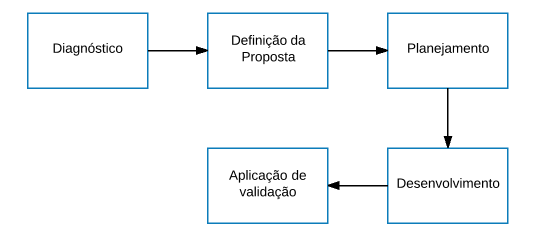
\includegraphics[scale=0.6]{figuras/etapas.png}
\caption{Etapas do trabalho}
\label{fig:etapas_trabalho}
\end{figure}

\noindent \textbf{Diagnóstico}: Esta etapa compreende o entendimento do escopo da plataforma ``Empurrando Juntos'' e do cenário das 
aplicações implementadas no contexto de violência contra a mulher.
% , por meio do levantamento dos sistemas relacionados e mapeamento
% de funcionalidades em comum.

\noindent \textbf{Definição da Proposta}: Nesta etapa há a definição da proposta do trabalho, o que compreende a definição de escopo, 
da arquitetura da API e da comunicação com o módulo de clusterização.

\noindent \textbf{Planejamento}: Nesta etapa há o planejamento da execução do trabalho com o estabelecimento
de um cronograma e do \textit{Roadmap}.

\noindent \textbf{Desenvolvimento}: Esta etapa compreende a realização de iterações para a implementação da API.

\noindent \textbf{Aplicação em um caso}: Esta etapa consiste na aplicação da API em uma plataforma de exemplo.

% Levantar sistemas relacionados, Mapear funcionalidades em comum, Definir escopo da API,
% Modelar estrutura da API, Desenvolver a API e Desenvolver um caso de exemplo.

% Passos: Levantar sistemas relacionados, definir escopo da api, definir tecnologia, 
% definir um questionário padrão a ser respondido pelas mulheres para apoio a tomada de decisão, implementar api, definir categorias, adicionar inteligência, definir ações

Nesse contexto, este trabalho está organizado em cinco capítulos. O Capítulo \ref{cap:clusterizacao} aborda os conceitos da técnica de 
classificação utilizada no ``Empurrando Juntos''. No Capítulo \ref{cap:api} são apresentados os conceitos e arquiteturas para APIs.
No Capítulo \ref{cap:sistemas_relacionados} são apresentados os sistemas existentes de apoio às mulheres vítimas de violência. A proposta do trabalho
é apresentada no Capítulo \ref{cap:proposta} e por fim são apresentadas as considerações finais no Capítulo \ref{cap:consideracoes_finais}.




